\section{Three experiments, one per clock}
\label{sec:experiments}

Each experiment below takes one concept from Table~\ref{tab:dictionary}, measures it on open models, and runs on a two-core CPU in under two hours. Details are in Appendix~\ref{app:details}, and the code reproduces every number.

\subsection{Experiment 1: the Lyapunov profile of the residual stream over training (clocks 1 and 2)}
\label{sec:exp1}

\paragraph{Question and setup.} Finite-time Lyapunov exponents \eqref{eq:ftle} describe how a forward pass stretches perturbations, layer by layer. How does this profile change as the model trains? This question couples clock~1 to clock~2 (\op{1}). We use the public training checkpoints of Pythia \citep{biderman2023pythia}: eleven checkpoints of Pythia-70M (6 layers), from initialization to step 143{,}000, and six checkpoints of Pythia-160M (12 layers). Each block is treated as a map $F_\ell$ on the full residual stream of a 16-token context. For each block we estimate the largest singular value $\sigma_\ell$ of its Jacobian by power iteration and report the relative exponent
\begin{equation}
\tilde\Lambda_\ell=\log\sigma_\ell-\log\big(\|x^{\ell+1}\|/\|x^{\ell}\|\big),
\end{equation}
which measures stretching beyond the growth of the residual norm. For the whole stack we report $\Lambda=\frac{1}{L}\log\sigma_{\max}(\mathrm{D}F_{0\to L})$, and the ratio $\kappa=\log\sigma_{\max}(\mathrm{D}F_{0\to L})/\sum_\ell\log\sigma_\ell$. Since $\sigma_{\max}$ of a product is at most the product of the $\sigma_\ell$, $\kappa\le1$ whenever $\sum_\ell\log\sigma_\ell>0$, which holds throughout our measurements, and $\kappa$ near one means that the most expanded direction of each layer is passed on to the next. Values are means over eight prompts, and $\kappa$ is the ratio of the two means.

\paragraph{Results.} Figure~\ref{fig:exp1} shows three things. First, at initialization both models have the same profile, decreasing with depth ($\tilde\Lambda_\ell$ from 1.20 to 0.53 in Pythia-70M and from 1.19 to 0.39 in Pythia-160M), which reflects the shared initialization scheme. Second, training makes every layer more expansive. The mean of $\tilde\Lambda_\ell$ over layers rises from 0.75 to 2.32 in Pythia-70M and from 0.59 to 2.17 in Pythia-160M, and it is still rising at the last checkpoint. The rise is not monotone at first: at step 128 the deepest layers of Pythia-70M contract further (layer 6 drops from 0.53 to 0.22) before all layers expand. Third, the whole stack does not follow. In Pythia-70M, $\Lambda$ goes from 0.87 to about 1.1 and stays between 1.11 and 1.18 from step 4{,}000 onward, which is under 3\% of training. In Pythia-160M it moves from 0.45 to 0.58. As a result the coherence $\kappa$ falls during training, from 0.67 to 0.36 in Pythia-70M and from 0.52 to 0.22 in Pythia-160M.

\paragraph{Reading.} Training produces layers that are individually more sensitive to perturbations, while the expanding directions of consecutive layers become less aligned, so the forward pass as a whole stretches perturbations only moderately. The depth-averaged exponent settles early, while the per-layer exponents keep changing. This is consistent with the observation that the normalized singular value spectra of the weights stabilize early in pretraining \citep{zhang2026stability}, now seen through the Jacobians of the forward map. These are measurements on two small models with short contexts and a small prompt set. Whether the same pattern holds at scale, and whether $\kappa$ predicts robustness to perturbations or the success of model editing, is part of \op{1}.

\begin{figure}[t]
\centering
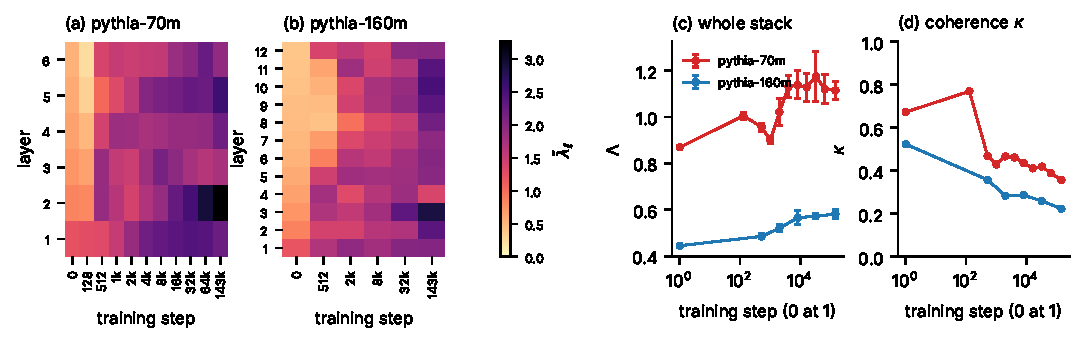
\includegraphics[width=\textwidth]{figs/exp1_ftle.pdf}
\caption{Experiment 1: finite-time Lyapunov exponents of the residual stream across public Pythia checkpoints. (a, b) Relative per-layer exponent $\tilde\Lambda_\ell$ (stretching of the top singular direction beyond the growth of the residual norm) for each layer and checkpoint. (c) Depth-averaged exponent of the whole stack, $\Lambda$; bars: standard deviation over prompts. (d) Coherence $\kappa$ between per-layer and whole-stack stretching; values below one mean that the most expanded directions of consecutive layers are not aligned.}
\label{fig:exp1}
\end{figure}


\subsection{Experiment 2: a learning-rate bifurcation diagram (clock 2)}
\label{sec:exp2}

\paragraph{Question and setup.} How does the long-run behavior of gradient descent on a transformer change with the step size $\eta$? We train a one-block transformer (two heads, width 32) with full-batch gradient descent on next-token prediction of sequences from a fixed random Markov chain, for 56 step sizes between $0.02$ and $4$. Within one seed every step size starts from the same initialization and sees the same data, and we repeat the sweep for three seeds that change both. Full batches remove minibatch noise, so any irregularity comes from the map \eqref{eq:clock2} itself. For each run we record the last 400 losses and the sharpness $\lambda_{\max}$ at the end.

\paragraph{Results.} Figure~\ref{fig:exp2} shows three regimes. In each seed, 48 of the 56 step sizes train. Across these 144 runs the final sharpness sits just above the stability threshold, with $\eta\lambda_{\max}/2$ having median $1.07$ and range $[1.00,1.21]$ across two decades of step size (panel b). This is the edge-of-stability behavior of \citet{cohen2021gradient}, and in this model it holds over the entire trainable range we tested. None of the runs settles on a fixed point. Removing the slow downward trend of the loss shows what the iterate does instead (panels a and c). For $\eta<0.05$ the fluctuations alternate in sign at every step, a period-2 orbit riding on the slow descent, and the median lag-1 autocorrelation of the detrended loss over the ten smallest step sizes is $-0.99$, $-0.99$ and $-0.97$ in the three seeds. As $\eta$ grows the fluctuations become larger and less regular. The median lag-1 autocorrelation rises to between $-0.95$ and $-0.92$ for $0.05\le\eta<0.3$, between $-0.74$ and $-0.68$ for $0.3\le\eta<1$, and between $-0.66$ and $-0.32$ for $\eta\ge1$. The edge of trainability depends on the seed. In seed 0 every $\eta\ge2.04$ diverges, while in seeds 1 and 2 divergent and trainable step sizes interleave between $1.5$ and $2.5$, and in seed 1 the largest trainable step size (2.47) lies above the smallest divergent one (1.68).

\paragraph{Reading.} In dictionary terms, the trainable range of this model is a sequence from a period-2 orbit near the stability boundary, through increasingly irregular oscillation, to divergence. This is the picture that minimal models predict \citep{chen2022edge,zhu2022edgeofstability,kong2020stochasticity}, here measured on a transformer with attention and layer normalization. The interleaving of trainable and divergent step sizes near the edge is consistent with the fractal trainability boundary reported by \citet{sohldickstein2024boundary}, although a grid of 56 points cannot measure a fractal dimension. We do not claim a full period-doubling cascade, since with 400-step tails on top of a slowly drifting loss we cannot resolve periods above two.

\begin{figure}[t]
\centering
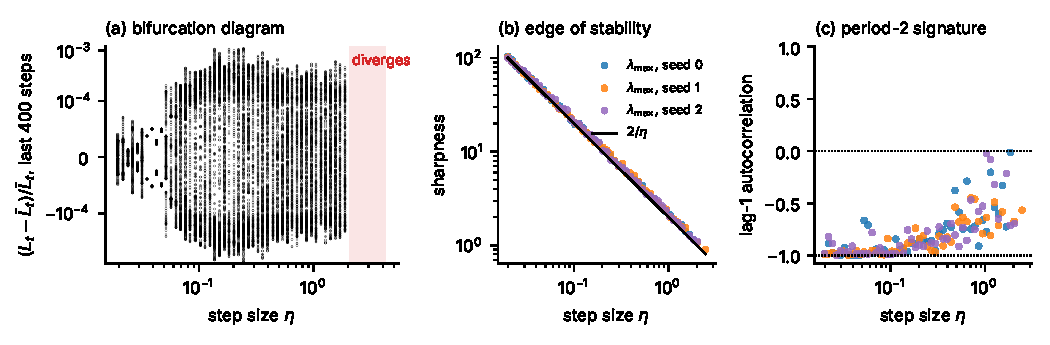
\includegraphics[width=\textwidth]{figs/exp2_bifurcation.pdf}
\caption{Experiment 2: full-batch gradient descent on a one-block transformer. (a) Bifurcation diagram for seed 0: relative deviation of the last 400 losses from their running mean (9-step window, symmetric-log axis) against the step size. Two branches at small $\eta$ mark a period-2 orbit; the band at larger $\eta$ is irregular oscillation; the shaded region diverges. (b) Sharpness at the end of training against $2/\eta$ for three seeds. (c) Lag-1 autocorrelation of the detrended loss for the same runs; $-1$ is a clean period-2 orbit.}
\label{fig:exp2}
\end{figure}

\subsection{Experiment 3: escape from repetition loops (clock 3)}
\label{sec:exp3}

\paragraph{Question and setup.} Section~\ref{sec:loops} predicts that escape from a repetition loop follows an Arrhenius law with the logit gap as barrier (Proposition~\ref{prop:arrhenius}), and that loops lock if the barrier grows from cycle to cycle (Proposition~\ref{prop:lock}). We test both on GPT-2 small \citep{radford2019language} and on the final checkpoint of Pythia-160M \citep{biderman2023pythia}. From each of 40 prompts we decode greedily for 320 tokens and keep the runs that end in a loop. Because the context along a loop is deterministic, the logits stored during the greedy run give the exact probability of staying in the loop at any temperature, and we check these exact values against Monte Carlo sampling.

\paragraph{Results.} Greedy decoding ends in a loop for 37 of the 40 prompts in each model, with periods from 4 to 53 tokens (median 23) in GPT-2 and from 7 to 46 tokens (median 22) in Pythia-160M (Figure~\ref{fig:exp3}).

The barrier grows. The median smallest logit gap $\Delta_c$ rises from 0.36 in the second cycle of a loop to 2.33 in the sixth and 3.63 in the twentieth in GPT-2, and from 0.47 to 1.83 and then 2.77 by the tenth cycle in Pythia-160M (panel a). The barrier in cycle 6 is larger than in cycle 2 for 36 of 36 GPT-2 loops and 35 of 37 Pythia-160M loops. This is the self-reinforcement reported by \citet{xu2022learning}, measured here as the depth of a well.

Escape follows the Arrhenius law. For the first cycle after two cycles of burn-in, the escape probability per cycle approaches $e^{-\Delta_{\min}/T}$ at low temperature (panel b). Fitting $\log r$ against $1/T$ recovers the measured barrier with a correlation of 0.997 in both models and a median relative difference of 6.9\% (22 GPT-2 loops) and 5.7\% (21 Pythia-160M loops). Loops whose escape probability never falls below $10^{-2}$ on our temperature grid are excluded from the fit (panel c). The exact survival probabilities agree with Monte Carlo sampling. Across 24 comparisons per model (four loops, two temperatures, survival after 1, 2 and 4 cycles, 128 samples each), the largest absolute difference is 0.062 for GPT-2 and 0.068 for Pythia-160M, and every difference is within two binomial standard errors.

Loops lock below a fairly sharp temperature. The median probability of staying in a loop until the end of the 320-token horizon is 0.89 at $T=0.31$ in both models, crosses 0.5 at $T\approx0.53$ (GPT-2) and $T\approx0.48$ (Pythia-160M), and falls to 0.06 and 0.015 at $T=0.75$ (panel d). Free sampling gives a consistent picture. After 200 tokens, 80\% (GPT-2) and 82.5\% (Pythia-160M) of generations end in a loop at $T=0.3$, 50\% and 35\% at $T=0.5$, at most 7.5\% at $T=0.7$, and none at $T\ge0.85$.

\paragraph{Reading.} The escape problem on clock~3 has the structure of Kramers' problem, with two differences that matter. The noise acts on a discrete choice through a Gibbs distribution, so the Arrhenius form follows directly from the softmax (Proposition~\ref{prop:arrhenius}) and needs no diffusion approximation. In addition, the barrier is a function of the residence time, so a loop becomes harder to leave the longer the model repeats it. Panel (a) also shows that the deepening is not uniform, and barriers often rise quickly over the first five cycles, pause, and rise again. Escape from a well whose depth grows with the time already spent in it is a non-stationary escape problem. Its mechanical analogue is a particle in a well that deepens as the particle settles, and its scaling with model size is open (\op{5}).

\begin{figure}[t]
\centering
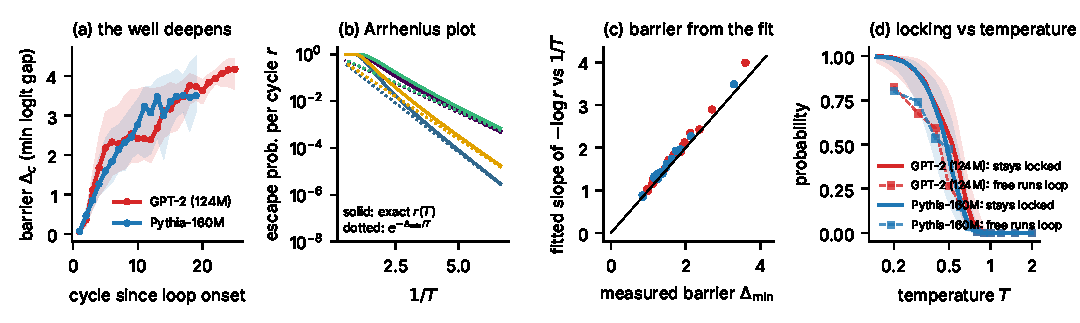
\includegraphics[width=\textwidth]{figs/exp3_escape.pdf}
\caption{Experiment 3: escape from repetition loops. (a) Barrier $\Delta_c$ (smallest logit gap in cycle $c$) against cycles since loop onset; line: median over loops, band: interquartile range; only cycles reached by at least 10 loops are shown. (b) Exact escape probability per cycle for four GPT-2 loops (solid) and the Arrhenius term $e^{-\Delta_{\min}/T}$ (dotted). (c) Barrier recovered from the slope of $\log r$ against $1/T$ at low temperature, against the measured $\Delta_{\min}$; line: identity. (d) Solid: median probability of staying in the loop until the end of the 320-token horizon, after two cycles of burn-in (band: interquartile range); the number of remaining cycles differs between loops because their onsets differ. Dashed: fraction of free generations of 200 tokens that end in a loop.}
\label{fig:exp3}
\end{figure}
